% TODO: OpenSSL tool, URLs, etc
\chapterold{Encrypted database case \#1}
\label{encrypted_DB1}

(This part has been first appeared in my blog at 26-Aug-2015.
Some discussion: \url{https://news.ycombinator.com/item?id=10128684}.)

\sectionold{Base64 and entropy}

\myindex{XML}
I've got the XML file containing some encrypted data.
It's probably related to some orders and/or customers information.

\begin{lstlisting}
<?xml version = "1.0" encoding = "UTF-8"?>
<Orders>
	<Order>
		<OrderID>1</OrderID>
		<Data>yjmxhXUbhB/5MV45chPsXZWAJwIh1S0aD9lFn3XuJMSxJ3/E+UE3hsnH</Data>
	</Order>
	<Order>
		<OrderID>2</OrderID>
		<Data>0KGe/wnypFBjsy+U0C2P9fC5nDZP3XDZLMPCRaiBw9OjIk6Tu5U=</Data>
	</Order>
	<Order>
		<OrderID>3</OrderID>
		<Data>mqkXfdzvQKvEArdzh+zD9oETVGBFvcTBLs2ph1b5bYddExzp</Data>
	</Order>
	<Order>
		<OrderID>4</OrderID>
		<Data>FCx6JhIDqnESyT3HAepyE1BJ3cJd7wCk+APCRUeuNtZdpCvQ2MR/7kLXtfUHuA==</Data>
	</Order>
...
\end{lstlisting}

The file is available \href{https://raw.githubusercontent.com/dennis714/yurichev.com/master/blog/encrypted_DB_case_1/encrypted.xml}{here}.

\myindex{base64}
This is clearly base64-encoded data, because all strings consisting of Latin characters, digits,
plus (+) and slash (/) symbols.
There can be 1 or 2 padding symbols (=), but they are never occurred in the middle of string.
Keeping in mind these base64 properties, it's very easy to recognize them.

Let's decode them and calculate entropies (\myref{entropy}) of these blocks in Wolfram Mathematica:

\begin{lstlisting}
In[]:= ListOfBase64Strings = 
  Map[First[#[[3]]] &, Cases[Import["encrypted.xml"], XMLElement["Data", _, _], Infinity]];

In[]:= BinaryStrings = 
  Map[ImportString[#, {"Base64", "String"}] &, ListOfBase64Strings];

In[]:= Entropies = Map[N[Entropy[2, #]] &, BinaryStrings];

In[]:= Variance[Entropies]
Out[]= 0.0238614
\end{lstlisting}

\myindex{Variance}
Variance is low.
This mean the entropy values are not very different from each other.
This is visible on graph:

\begin{lstlisting}
In[]:= ListPlot[Entropies]
\end{lstlisting}

\begin{figure}[H]
\centering
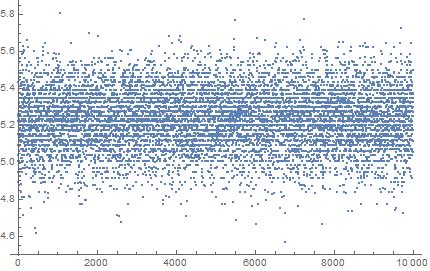
\includegraphics[scale=\FigScale]{examples/encrypted_DB1/entropy.png}
\end{figure}

Most valuess are between 5.0 and 5.4.
This is a sign that the data is compressed and/or encrypted.

To understand variance, let's calculate entropies of all lines in Conan Doyle's \IT{The Hound of the Baskervilles} book:

\begin{lstlisting}
In[]:= BaskervillesLines = Import["http://www.gutenberg.org/cache/epub/2852/pg2852.txt", "List"];

In[]:= EntropiesT = Map[N[Entropy[2, #]] &, BaskervillesLines];

In[]:= Variance[EntropiesT]
Out[]= 2.73883

In[]:= ListPlot[EntropiesT]
\end{lstlisting}

\begin{figure}[H]
\centering
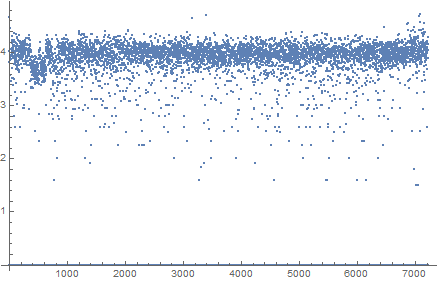
\includegraphics[scale=\FigScale]{examples/encrypted_DB1/conan_doyle.png}
\end{figure}

Most values are gathered around value of 4, but there are also values which are smaller,
and they are influenced final variance value.

Perhaps, shortest strings has smaller entropy, let's take short string from the Conan Doyle's book:

\begin{lstlisting}
In[]:= Entropy[2, "Yes, sir."] // N
Out[]= 2.9477
\end{lstlisting}

Let's try even shorter:

\begin{lstlisting}
In[]:= Entropy[2, "Yes"] // N
Out[]= 1.58496

In[]:= Entropy[2, "No"] // N
Out[]= 1.
\end{lstlisting}

\sectionold{Is it compressed?}

OK, so our data is compressed and/or encrypted.
Is it compressed? Almost all data compressors put some header at the start, signature, or something like that.
As we can see, there are no consistent data at the start.
It's still possible that this is DIY handmade data compressor, but they are very rare.
Handmade cryptoalgorithm is very easy implement because it's very easy to make it work.
\myindex{memfrob()}
\myindex{ROT13}
Even primitive keyless cryptosystems like \IT{memfrob()}\footnote{\url{http://linux.die.net/man/3/memfrob}}
and ROT13 working fine without errors.
It's a challenge to write data compressor from scratch using only fantasy and imagination in a way so it will have no evident bugs.
Some programmers implements data compression functions by reading textbooks, but this is also rare.
The most popular two ways are:
\myindex{zlib}
1) just take open-source library like zlib;
2) copy\&paste something from somewhere.
Open-source data compressions algorithms usually puts some kind of header, and so
are popular code snippets from the sites like \url{http://www.codeproject.com/}.

\sectionold{Is it encrypted?}

All major data encryption algorithms process data in blocks. DES---8 bytes, AES---16 bytes.
If the input buffer is not divided evenly by block, it's padded, so encrypted data is aligned
by cryptoalgorithm's block size.
This is not our case.

Using Wolfram Mathematica, I analyzed data block's lengths:

\begin{lstlisting}
In[]:= Counts[Map[StringLength[#] &, BinaryStrings]]
Out[]= <|42 -> 1858, 38 -> 1235, 36 -> 699, 46 -> 1151, 40 -> 1784, 
 44 -> 1558, 50 -> 366, 34 -> 291, 32 -> 74, 56 -> 15, 48 -> 716, 
 30 -> 13, 52 -> 156, 54 -> 71, 60 -> 3, 58 -> 6, 28 -> 4|>
\end{lstlisting}

1858 blocks has size of 42 bytes, 1235 blocks has size of 38 bytes, etc.

I made a graph:

\begin{lstlisting}
ListPlot[Counts[Map[StringLength[#] &, BinaryStrings]]]
\end{lstlisting}

\begin{figure}[H]
\centering
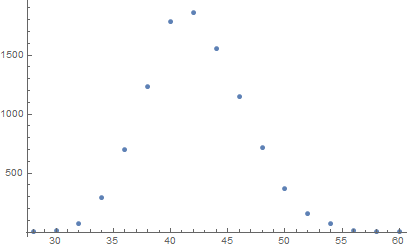
\includegraphics[scale=\FigScale]{examples/encrypted_DB1/lengths.png}
\end{figure}

So, most blocks has size between ~36 and ~48.
There is also another thing to notice: all block sizes are even.
No single block with odd size.

There are, however, stream ciphers which can operate on byte or bit-level.

\sectionold{CryptoPP}
\myindex{CryptoPP}

The program which can browse this encrypted database is written C\# and the .NET code
is heavily obfuscated.
Nevertheless, there is DLL with x86 code, which, after brief examination,
has parts of the CryptoPP popular open-source library!
(I just spotted "CryptoPP" strings inside.)
Now it's very easy to find all functions inside of DLL because CryptoPP library is open-source.

\myindex{AES}
CryptoPP library has a lot of crypto-functions, including AES (AKA Rijndael).
Newer x86 CPUs has AES helper instructions like AESENC, AESDEC and AESKEYGENASSIST
\footnote{\url{https://en.wikipedia.org/wiki/AES_instruction_set}}.
They are not performing encryption/decryption completely, but they do significant amount of job.
And newer CryptoPP versions use them.
For example, here:
\href{https://github.com/mmoss/cryptopp/blob/2772f7b57182b31a41659b48d5f35a7b6cedd34d/src/rijndael.cpp#L1034}{1},
\href{https://github.com/mmoss/cryptopp/blob/2772f7b57182b31a41659b48d5f35a7b6cedd34d/src/rijndael.cpp#L1000}{2}.
\myindex{x86!\Instructions!AESENC}
\myindex{x86!\Instructions!AESDEC}
\myindex{tracer}
To my surprise, during decryption, AESENC is executed, while AESDEC is not 
(I just checked with my tracer utility, but any debugger can be used).
I checked, if my CPU really supports AES instructions. Some Intel i3 CPUs are not.
And if not, CryptoPP library falling back to AES functions implemented in old way
\footnote{\url{https://github.com/mmoss/cryptopp/blob/2772f7b57182b31a41659b48d5f35a7b6cedd34d/src/rijndael.cpp#L355}}.
But my CPU supports them.
Why AESDEC is still not executed?
Why the program use AES encryption in order to decrypt database?

OK, it's not a problem to find a function which encrypts block.
It is called \IT{CryptoPP::Rijndael::Enc::ProcessAndXorBlock}:
\url{https://github.com/mmoss/cryptopp/blob/2772f7b57182b31a41659b48d5f35a7b6cedd34d/src/rijndael.cpp#L349},
and it has references to another function: \IT{Rijndael::Enc::AdvancedProcessBlocks()}
\url{https://github.com/mmoss/cryptopp/blob/2772f7b57182b31a41659b48d5f35a7b6cedd34d/src/rijndael.cpp#L1179},
which, in turn, has references to two functions (
\href{https://github.com/mmoss/cryptopp/blob/2772f7b57182b31a41659b48d5f35a7b6cedd34d/src/rijndael.cpp#L1000}{AESNI\_Enc\_Block}
and 
\href{https://github.com/mmoss/cryptopp/blob/2772f7b57182b31a41659b48d5f35a7b6cedd34d/src/rijndael.cpp#L1012}{AESNI\_Enc\_4\_Blocks}
)
which has AESENC instructions.

So, judging by CryptoPP internals, \IT{CryptoPP::Rijndael::Enc::ProcessAndXorBlock()} encrypts one 16-byte block.
Let's set breakpoint on it and see, what happens during decryption.
I use my simple tracer tool again.
The software should decrypt first data block now.
Oh, by the way, here is the first data block converted from base64 encoding to hexadecimal data,
let's have it at hand:

\lstinputlisting{examples/encrypted_DB1/1.lst}

This is also arguments of the function from CryptoPP source files:

\begin{lstlisting}
size_t Rijndael::Enc::AdvancedProcessBlocks(const byte *inBlocks, const byte *xorBlocks, byte *outBlocks, size_t length, word32 flags);
\end{lstlisting}

So it has 5 arguments. Possible flags are:

\begin{lstlisting}
enum {BT_InBlockIsCounter=1, BT_DontIncrementInOutPointers=2, BT_XorInput=4, BT_ReverseDirection=8, BT_AllowParallel=16} FlagsForAdvancedProcessBlocks;
\end{lstlisting}

OK, run tracer on \IT{ProcessAndXorBlock()} function:

\lstinputlisting{examples/encrypted_DB1/2.lst}

Here we can see inputs and outputs to the \IT{ProcessAndXorBlock()} function.

This is output from the first call of encryption operation:

\begin{lstlisting}
00000000: C7 39 4E 7B 33 1B D6 1F-B8 31 10 39 39 13 A5 5D ".9N{3....1.99..]"
\end{lstlisting}

Then the \IT{ProcessAndXorBlock()} is called with 0-length block, but with 8 flag (\IT{BT\_ReverseDirection}).

Second:

\begin{lstlisting}
00000000: 45 00 20 00 4A 00 4F 00-48 00 4E 00 53 00 00 00 "E. .J.O.H.N.S..."
\end{lstlisting}

Wow, there is some string familiar to us!

Third:

\begin{lstlisting}
00000000: B1 27 7F E4 9F 01 E3 81-CF C6 12 FB B9 7C F1 BC ".'...........|.."
\end{lstlisting}

The first output is very similar to the first 16 bytes of the encrypted buffer.

Output of the first call of \IT{ProcessAndXorBlock()}:

\begin{lstlisting}
00000000: C7 39 4E 7B 33 1B D6 1F-B8 31 10 39 39 13 A5 5D ".9N{3....1.99..]"
\end{lstlisting}

First 16 bytes of encrypted buffer:

\begin{lstlisting}
00000000: CA 39 B1 85 75 1B 84 1F F9 31 5E 39 72 13 EC 5D  .9..u....1^9r..]
\end{lstlisting}

There are too much equal bytes!
How AES encryption result can be very similar to the encrypted buffer while this is not
encryption but rather decryption?!

\sectionold{Cipher Feedback mode}

\myindex{Cipher Feedback mode}
\myindex{XOR}
The answer is CFB (Cipher Feedback mode):
In this mode, AES algorithms used not as encryption algorithm, but as a device which generates cryptographically secure random data.
The actual encryption is happens using simple XOR operation.

Here is encryption algorithm (images are taken from Wikipedia):

\begin{figure}[H]
\centering
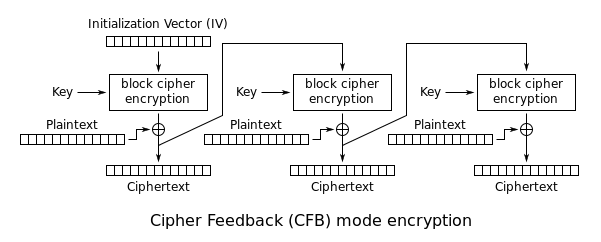
\includegraphics[scale=\FigScale]{examples/encrypted_DB1/601px-CFB_encryption.svg.png}
\end{figure}

And decryption:

\begin{figure}[H]
\centering
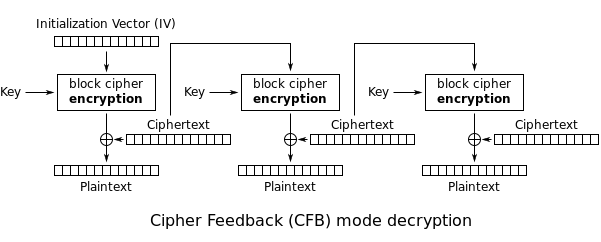
\includegraphics[scale=\FigScale]{examples/encrypted_DB1/601px-CFB_decryption.svg.png}
\label{fig:CFB_decryption}
\end{figure}

Now let's see: AES encryption operation generates 16 bytes (or 128 bits) or \IT{random} data
to be used while XOR-ing, who forces us to use all 16 bytes?
If at the last stage we've got 1 byte of data, let's xor 1 byte of data with 1 byte of generated
\IT{random} data?
This leads to important property of CFB mode: data must not be padded, data of arbitrary size
can be encrypted and decrypted.

Oh, that's why all encrypted blocks are not padded.
And that's why AESDEC instruction is never called.

Let's try to decrypt first block manually, using Python.
CFB mode also use IV (initialization vector), as a \IT{seed} to \IT{random generator}.
In our case, IV is the block which is encrypted at first stage:

\begin{lstlisting}
0038B920: 01 00 00 00 FF FF FF FF-79 C1 69 0B 67 C1 04 7D "........y.i.g..}"
\end{lstlisting}

Oh, and we also need to recover encryption key.
\myindex{x86!\Instructions!AESKEYGENASSIST}
There is AESKEYGENASSIST is DLL, and it is called, and it is used in the 
\IT{Rijndael::Base::UncheckedSetKey()} function:
\url{https://github.com/mmoss/cryptopp/blob/2772f7b57182b31a41659b48d5f35a7b6cedd34d/src/rijndael.cpp#L198}
It's easy to find it in IDA and set breakpoint. Let's see:

\begin{lstlisting}
... tracer.exe -l:filename.exe bpf=filename.exe!0x435c30,args:3,dump_args:0x10

Warning: no tracer.cfg file.
PID=2068|New process software.exe
no module registered with image base 0x77320000
no module registered with image base 0x76e20000
no module registered with image base 0x77320000
no module registered with image base 0x77220000
Warning: unknown (to us) INT3 breakpoint at ntdll.dll!LdrVerifyImageMatchesChecksum+0x96c (0x776c103b)
(0) software.exe!0x435c30(0x15e8000, 0x10, 0x14f808) (called from software.exe!.text+0x22fa1 (0x13d3fa1))
Argument 1/3 
015E8000: CD C5 7E AD 28 5F 6D E1-CE 8F CC 29 B1 21 88 8E "..~.(_m....).!.."
Argument 3/3 
0014F808: 38 82 58 01 C8 B9 46 00-01 D1 3C 01 00 F8 14 00 "8.X...F...<....."
Argument 3/3 +0x0: software.exe!.rdata+0x5238
Argument 3/3 +0x8: software.exe!.text+0x1c101
(0) software.exe!0x435c30() -> 0x13c2801
PID=2068|Process software.exe exited. ExitCode=0 (0x0)
\end{lstlisting}

So this is the key: \IT{CD C5 7E AD 28 5F 6D E1-CE 8F CC 29 B1 21 88 8E}.

During manual decryption we've got this:

\begin{lstlisting}
00000000: 0D 00 FF FE 46 00 52 00  41 00 4E 00 4B 00 49 00  ....F.R.A.N.K.I.
00000010: 45 00 20 00 4A 00 4F 00  48 00 4E 00 53 00 66 66  E. .J.O.H.N.S.ff
00000020: 66 66 66 9E 61 40 D4 07  06 01                    fff.a@....
\end{lstlisting}

Now this is something readable!
And now we can see why there were so many equal bytes at the first decryption stage:
because plaintext has so many zero bytes!

Let's decrypt the second block:

\begin{lstlisting}
00000000: 17 98 D0 84 3A E9 72 4F  DB 82 3F AD E9 3E 2A A8  ....:.rO..?..>*.
00000010: 41 00 52 00 52 00 4F 00  4E 00 CD CC CC CC CC CC  A.R.R.O.N.......
00000020: 1B 40 D4 07 06 01                                 .@....
\end{lstlisting}

Third, fourth and fifth:

\begin{lstlisting}
00000000: 5D 90 59 06 EF F4 96 B4  7C 33 A7 4A BE FF 66 AB  ].Y.....|3.J..f.
00000010: 49 00 47 00 47 00 53 00  00 00 00 00 00 C0 65 40  I.G.G.S.......e@
00000020: D4 07 06 01                                       ....
\end{lstlisting}

\begin{lstlisting}
00000000: D3 15 34 5D 21 18 7C 6E  AA F8 2D FE 38 F9 D7 4E  ..4]!.|n..-.8..N
00000010: 41 00 20 00 44 00 4F 00  48 00 45 00 52 00 54 00  A. .D.O.H.E.R.T.
00000020: 59 00 48 E1 7A 14 AE FF  68 40 D4 07 06 02        Y.H.z...h@....
\end{lstlisting}

\begin{lstlisting}
00000000: 1E 8B 90 0A 17 7B C5 52  31 6C 4E 2F DE 1B 27 19  .....{.R1lN...'.
00000010: 41 00 52 00 43 00 55 00  53 00 00 00 00 00 00 60  A.R.C.U.S.......
00000020: 66 40 D4 07 06 03                                 f@....
\end{lstlisting}

All blocks decrypted seems correctly except of first 16 byte part.

\sectionold{Initializing Vector}

What can affect first 16 bytes?

Let's back to CFB decryption algorithm again: \myref{fig:CFB_decryption}.

We can see that IV can affect to first block decryption operation, but not the second,
because the second stage used ciphertext from the first stage, and in case of decryption,
it's the same, no matter what IV has!

So probably, IV is different each time.
Using my tracer, I'll take a look at the first input during decryption of the second block
of XML file:

\begin{lstlisting}
0038B920: 02 00 00 00 FE FF FF FF-79 C1 69 0B 67 C1 04 7D "........y.i.g..}"
\end{lstlisting}

... third:

\begin{lstlisting}
0038B920: 03 00 00 00 FD FF FF FF-79 C1 69 0B 67 C1 04 7D "........y.i.g..}"
\end{lstlisting}

It seems, first and fifth byte are changed each time.
I finally concluded that the first 32-bit integer is just OrderID from the XML file,
and the second is also OrderID, but negated. All other 8 bytes are static.
Now I have decrypted the whole database: 
\url{https://raw.githubusercontent.com/dennis714/yurichev.com/master/blog/encrypted_DB_case_1/decrypted.full.txt}.

The Python script used for this is: 
\url{https://github.com/dennis714/yurichev.com/blob/master/blog/encrypted_DB_case_1/decrypt_blocks.py}.

Perhaps, author wanted each block encrypted differently, so he/she used OrderID as part of key.
It would be also possible to make different AES key instead of IV.

So now we know that IV only affects first block during decryption in CFB mode, this is
feature of it.
All other blocks can be decrypted without knowledge IV, but using the key.

OK, so why CFB mode? Apparently, because the very first AES example on CryptoPP wiki
uses CFB mode: 
\url{http://www.cryptopp.com/wiki/Advanced_Encryption_Standard#Encrypting_and_Decrypting_Using_AES}.
Supossedly, CryptoPP developers choose it for simplicity: 
the example can encrypt/decrypt text strings with arbitrary lengths, without padding.

It is very likely, my program's programmer(s) just copypasted the example from CryptoPP wiki page.
Many programmers do so.

The only difference that IV is choosen randomly in CryptoPP wiki example, while this indeterminism
wasn't allowable to programmers of the software we are dissecting now, 
so they choose to initialize IV using Order ID.

Now we can proceed to analyzing matter of each byte in the decrypted block.

\sectionold{Structure of the buffer}

Let's take first four decrypted blocks:

\begin{lstlisting}
00000000: 0D 00 FF FE 46 00 52 00  41 00 4E 00 4B 00 49 00  ....F.R.A.N.K.I.
00000010: 45 00 20 00 4A 00 4F 00  48 00 4E 00 53 00 66 66  E. .J.O.H.N.S.ff
00000020: 66 66 66 9E 61 40 D4 07  06 01                    fff.a@....

00000000: 0B 00 FF FE 4C 00 4F 00  52 00 49 00 20 00 42 00  ....L.O.R.I. .B.
00000010: 41 00 52 00 52 00 4F 00  4E 00 CD CC CC CC CC CC  A.R.R.O.N.......
00000020: 1B 40 D4 07 06 01                                 .@....

00000000: 0A 00 FF FE 47 00 41 00  52 00 59 00 20 00 42 00  ....G.A.R.Y. .B.
00000010: 49 00 47 00 47 00 53 00  00 00 00 00 00 C0 65 40  I.G.G.S.......e@
00000020: D4 07 06 01                                       ....

00000000: 0F 00 FF FE 4D 00 45 00  4C 00 49 00 4E 00 44 00  ....M.E.L.I.N.D.
00000010: 41 00 20 00 44 00 4F 00  48 00 45 00 52 00 54 00  A. .D.O.H.E.R.T.
00000020: 59 00 48 E1 7A 14 AE FF  68 40 D4 07 06 02        Y.H.z...h@....
\end{lstlisting}

UTF-16 encoded text strings are clearly visible, these are names and surnames.
The first byte (or 16-bit word) is seems string length, we can visually check it.
\IT{FF FE} is seems Unicode \ac{BOM}.

There are 12 more bytes after each string.

Using this script 
(\url{https://github.com/dennis714/yurichev.com/blob/master/blog/encrypted_DB_case_1/dump_buffer_rest.py})
I've got random selection of the block \IT{tails}:

\lstinputlisting{examples/encrypted_DB1/tails.lst}

We first see the 0x40 and 0x07 bytes present in each \IT{tail}.
The very last byte s always in 1..0x1F (1..31) range, as I checked.
The penultimate byte is always in 1..0xC (1..12) range.
Wow, that looks like a date!
Year can be represented as 16-bit value, and maybe last 4 bytes is date (16 bits for year, 8 bits
for month and day)?
0x7DD is 2013, 0x7D5 is 2005, etc. Seems fine. This is a date.
There are 8 more bytes.
Judging by the fact this is database named \IT{orders}, maybe some kind of sum is present here?
I made attempt to interpret it as double-precision IEEE 754 floating point and dump all values!

Some are:

\begin{lstlisting}
71.0
134.0
51.95
53.0
121.99
96.95
98.95
15.95
85.95
184.99
94.95
29.95
85.0
36.0
130.99
115.95
87.99
127.95
114.0
150.95
\end{lstlisting}

Looks like real!

Now we can dump names, sums and dates.

\begin{lstlisting}
plain:
00000000: 0D 00 FF FE 46 00 52 00  41 00 4E 00 4B 00 49 00  ....F.R.A.N.K.I.
00000010: 45 00 20 00 4A 00 4F 00  48 00 4E 00 53 00 66 66  E. .J.O.H.N.S.ff
00000020: 66 66 66 9E 61 40 D4 07  06 01                    fff.a@....
OrderID= 1 name= FRANKIE JOHNS sum= 140.95 date= 2004 / 6 / 1

plain:
00000000: 0B 00 FF FE 4C 00 4F 00  52 00 49 00 20 00 42 00  ....L.O.R.I. .B.
00000010: 41 00 52 00 52 00 4F 00  4E 00 CD CC CC CC CC CC  A.R.R.O.N.......
00000020: 1B 40 D4 07 06 01                                 .@....
OrderID= 2 name= LORI BARRON sum= 6.95 date= 2004 / 6 / 1

plain:
00000000: 0A 00 FF FE 47 00 41 00  52 00 59 00 20 00 42 00  ....G.A.R.Y. .B.
00000010: 49 00 47 00 47 00 53 00  00 00 00 00 00 C0 65 40  I.G.G.S.......e@
00000020: D4 07 06 01                                       ....
OrderID= 3 name= GARY BIGGS sum= 174.0 date= 2004 / 6 / 1

plain:
00000000: 0F 00 FF FE 4D 00 45 00  4C 00 49 00 4E 00 44 00  ....M.E.L.I.N.D.
00000010: 41 00 20 00 44 00 4F 00  48 00 45 00 52 00 54 00  A. .D.O.H.E.R.T.
00000020: 59 00 48 E1 7A 14 AE FF  68 40 D4 07 06 02        Y.H.z...h@....
OrderID= 4 name= MELINDA DOHERTY sum= 199.99 date= 2004 / 6 / 2

plain:
00000000: 0B 00 FF FE 4C 00 45 00  4E 00 41 00 20 00 4D 00  ....L.E.N.A. .M.
00000010: 41 00 52 00 43 00 55 00  53 00 00 00 00 00 00 60  A.R.C.U.S.......
00000020: 66 40 D4 07 06 03                                 f@....
OrderID= 5 name= LENA MARCUS sum= 179.0 date= 2004 / 6 / 3
\end{lstlisting}

See more: \url{https://raw.githubusercontent.com/dennis714/yurichev.com/master/blog/encrypted_DB_case_1/decrypted.full.with_data.txt}.
Or filtered: \url{https://github.com/dennis714/yurichev.com/blob/master/blog/encrypted_DB_case_1/decrypted.short.txt}.
Seems correct.

This is some kind of OOP serialization, i.e., packing differently typed values into binary buffer for storing and/or transmitting.

\sectionold{Noise at the end}

The only thing is that sometimes, tail is bigger:

\begin{lstlisting}
00000000: 0E 00 FF FE 54 00 48 00  45 00 52 00 45 00 53 00  ....T.H.E.R.E.S.
00000010: 45 00 20 00 54 00 55 00  54 00 54 00 4C 00 45 00  E. .T.U.T.T.L.E.
00000020: 66 66 66 66 66 1E 63 40  D4 07 07 1A 00 07 07 19  fffff.c@........
OrderID= 172 name= THERESE TUTTLE sum= 152.95 date= 2004 / 7 / 26
\end{lstlisting}

(\IT{00 07 07 19} bytes are not used and is ballast).

\begin{lstlisting}
00000000: 0C 00 FF FE 4D 00 45 00  4C 00 41 00 4E 00 49 00  ....M.E.L.A.N.I.
00000010: 45 00 20 00 4B 00 49 00  52 00 4B 00 00 00 00 00  E. .K.I.R.K.....
00000020: 00 20 64 40 D4 07 09 02  00 02                    . d@......
OrderID= 286 name= MELANIE KIRK sum= 161.0 date= 2004 / 9 / 2
\end{lstlisting}

(\IT{00 02} are not used).

After close examination, we can see, that the noise at the end of tail is just left
from previous encryption!

Here are two subsequent buffers:

\begin{lstlisting}
00000000: 10 00 FF FE 42 00 4F 00  4E 00 4E 00 49 00 45 00  ....B.O.N.N.I.E.
00000010: 20 00 47 00 4F 00 4C 00  44 00 53 00 54 00 45 00   .G.O.L.D.S.T.E.
00000020: 49 00 4E 00 9A 99 99 99  99 79 46 40 D4 07 07 19  I.N......yF@....
OrderID= 171 name= BONNIE GOLDSTEIN sum= 44.95 date= 2004 / 7 / 25

00000000: 0E 00 FF FE 54 00 48 00  45 00 52 00 45 00 53 00  ....T.H.E.R.E.S.
00000010: 45 00 20 00 54 00 55 00  54 00 54 00 4C 00 45 00  E. .T.U.T.T.L.E.
00000020: 66 66 66 66 66 1E 63 40  D4 07 07 1A 00 07 07 19  fffff.c@........
OrderID= 172 name= THERESE TUTTLE sum= 152.95 date= 2004 / 7 / 26
\end{lstlisting}

(The last \IT{07 07 19} bytes are copied from the previous plaintext buffer).

Another two subsequent buffers:

\begin{lstlisting}
00000000: 0D 00 FF FE 4C 00 4F 00  52 00 45 00 4E 00 45 00  ....L.O.R.E.N.E.
00000010: 20 00 4F 00 54 00 4F 00  4F 00 4C 00 45 00 CD CC   .O.T.O.O.L.E...
00000020: CC CC CC 3C 5E 40 D4 07  09 02                    ...<^@....
OrderID= 285 name= LORENE OTOOLE sum= 120.95 date= 2004 / 9 / 2

00000000: 0C 00 FF FE 4D 00 45 00  4C 00 41 00 4E 00 49 00  ....M.E.L.A.N.I.
00000010: 45 00 20 00 4B 00 49 00  52 00 4B 00 00 00 00 00  E. .K.I.R.K.....
00000020: 00 20 64 40 D4 07 09 02  00 02                    . d@......
OrderID= 286 name= MELANIE KIRK sum= 161.0 date= 2004 / 9 / 2
\end{lstlisting}

The last 02 byte is copied from the previous plaintext buffer.

It's possible if the buffer used while encrypting was global and/or wasn't cleared before
each encryption.
The final buffer size value is also biased somehow, nevertheless, the bug left uncatched
because it doesn't affect decrypting software, it's just ignores noise at the end.
This is common mistake.
\myindex{OpenSSL}
\myindex{Heartbleed}
It even affected OpenSSL (Heartbleed bug).

\sectionold{Conclusion}

Summary:
every practicing reverse engineer should be familiar with major crypto algorithms and
also major cryptographical modes.
Some books about it: \myref{crypto_books}.

\IT{Encrypted} database contents has been artificially constructed by me for the sake of demonstation.
I've got most popular USA names and surnames from there: \url{http://stackoverflow.com/questions/1803628/raw-list-of-person-names},
and combined them randomly.
Dates and sums were also generated randomly.

All files used in this article are here: \url{https://github.com/dennis714/yurichev.com/tree/master/blog/encrypted_DB_case_1}.

Nevertheless, many features like these I've observed in real-world software applications.
This example is based on them.

\sectionold{Post Scriptum: brute-forcing IV}

The case you saw is artificially constructed, but based on some real applications I've observed.
When I've been working on one of such real applications, 
I first noticed that Initializing Vector (IV) is generating using some 32-bit number, I wasn't able to find a link between this value and OrderID.
So I prepared to use brute-force, which is indeed possible here.
It's not a problem to enumerate all 32-bit values and try each IV based on each.
Then you decrypt 16-byte block and check for zero bytes, which are always at fixed places.

